\section{Existing implementations}
\label{sect:existing_implementations}

This section describes some of the most interesting existing implementations of
XQuery parsers and translators. Note that some of these are fundamentally
different in some aspects (for example, eXist operates on DOM trees), but may
implement certain features of interest, and are therefore included here.

\subsection{eXist}
eXist\cite{exist_doc} is an open source native XML database with an XQuery
query processor. The eXist system is written in Java. This system stores native
XML data in B-trees and paged files, and document nodes
in persistent DOM trees\cite{exist_factsheet}. Document collections are stored
in a hierarchical manner similar to a regular file system.

eXist has a numerical indexing scheme for identification of relationships
between nodes (parent/child, ancestor/descendant, previous/next sibling). This
provides a structural index for element attribute nodes. In addition, eXist has
a fulltext index for text and attribute values, and range indexes for typed
values.

Based on these provided index types, the eXist XQuery engine relies on path
join algorithms\cite{exist_idx_drv_query} for efficient computation of node
relationships instead of traditional tree traversals. 

\subsection{Pathfinder}
\label{sect:theory:pathfinder}
\begin{figure}[h]
  \centering
    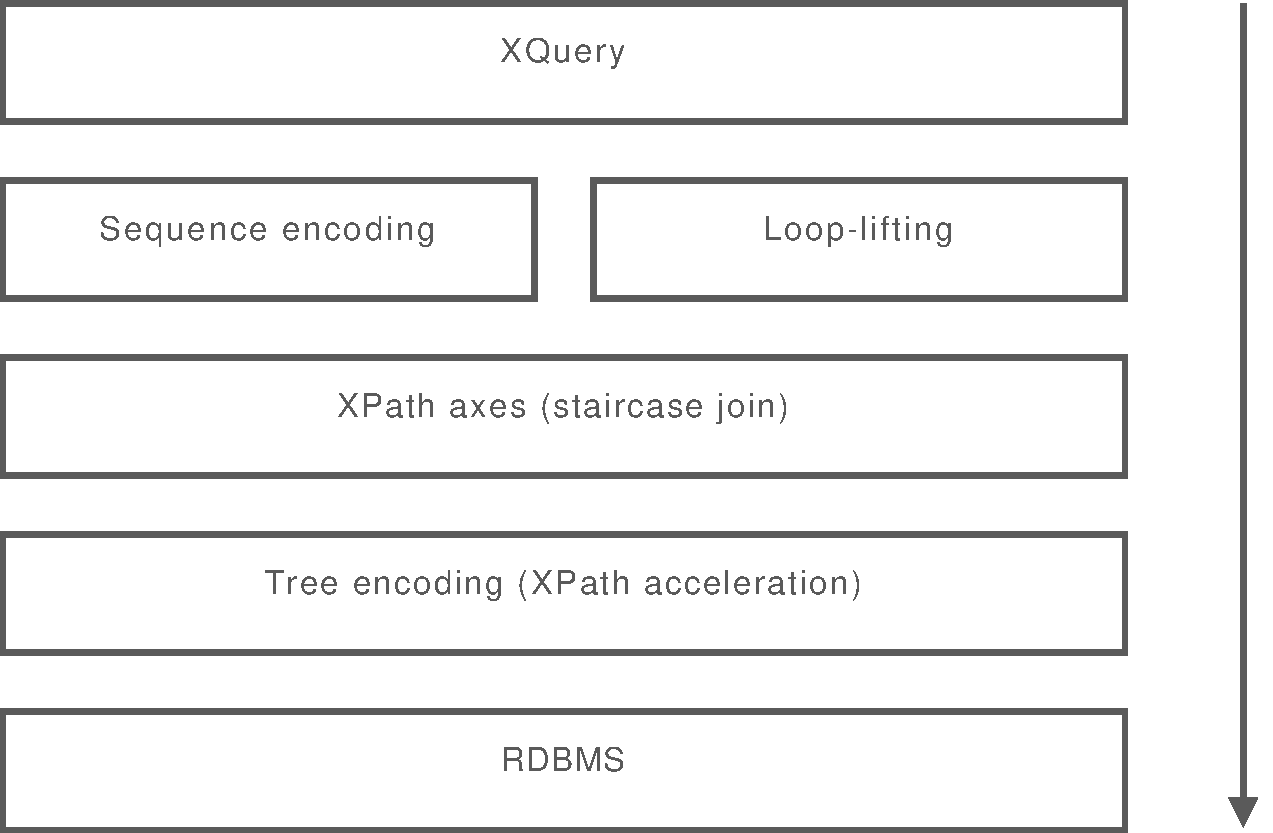
\includegraphics[width=0.6\textwidth]{diagrams/pathfinder_arch}
  \caption{Pathfinder architecture / development stack}
\end{figure}
Pathfinder\cite{pathfinderHome} claims to be a ``purely relational XQuery
processor'', which theoretically can utilise any off-the-shelf RBDMS as a
backend for XQuery execution in a relational context.

The technique for transforming XQuery into relational algebra is called ``Loop
Lifting''\cite{pathfinder_mothertongue}. Loop Lifting is a FLWOR-centric
approach which essentially transforms iterations into joins. The technique is
described in detail in section \ref{sect:trans:loop_lifting}.

As a relational backend, the XQuery processor uses MonetDB, an integrated
component in the Pathfinder project. However, recent versions of Pathfinder is
also capable of producing SQL code for execution on conventional database
systems. As a proof of concept, they performed the XMark test suite on top of
the IBM DB2 system\cite{pathfinder_sql}.

\textbf{\Large TODO:}
\begin{itemize}
  \item nevne staircase join
  \item hvordan de lagrer data
  \item forklare figuren
\end{itemize}

\subsection{Galatex}
\begin{figure}[h]
  \centering
    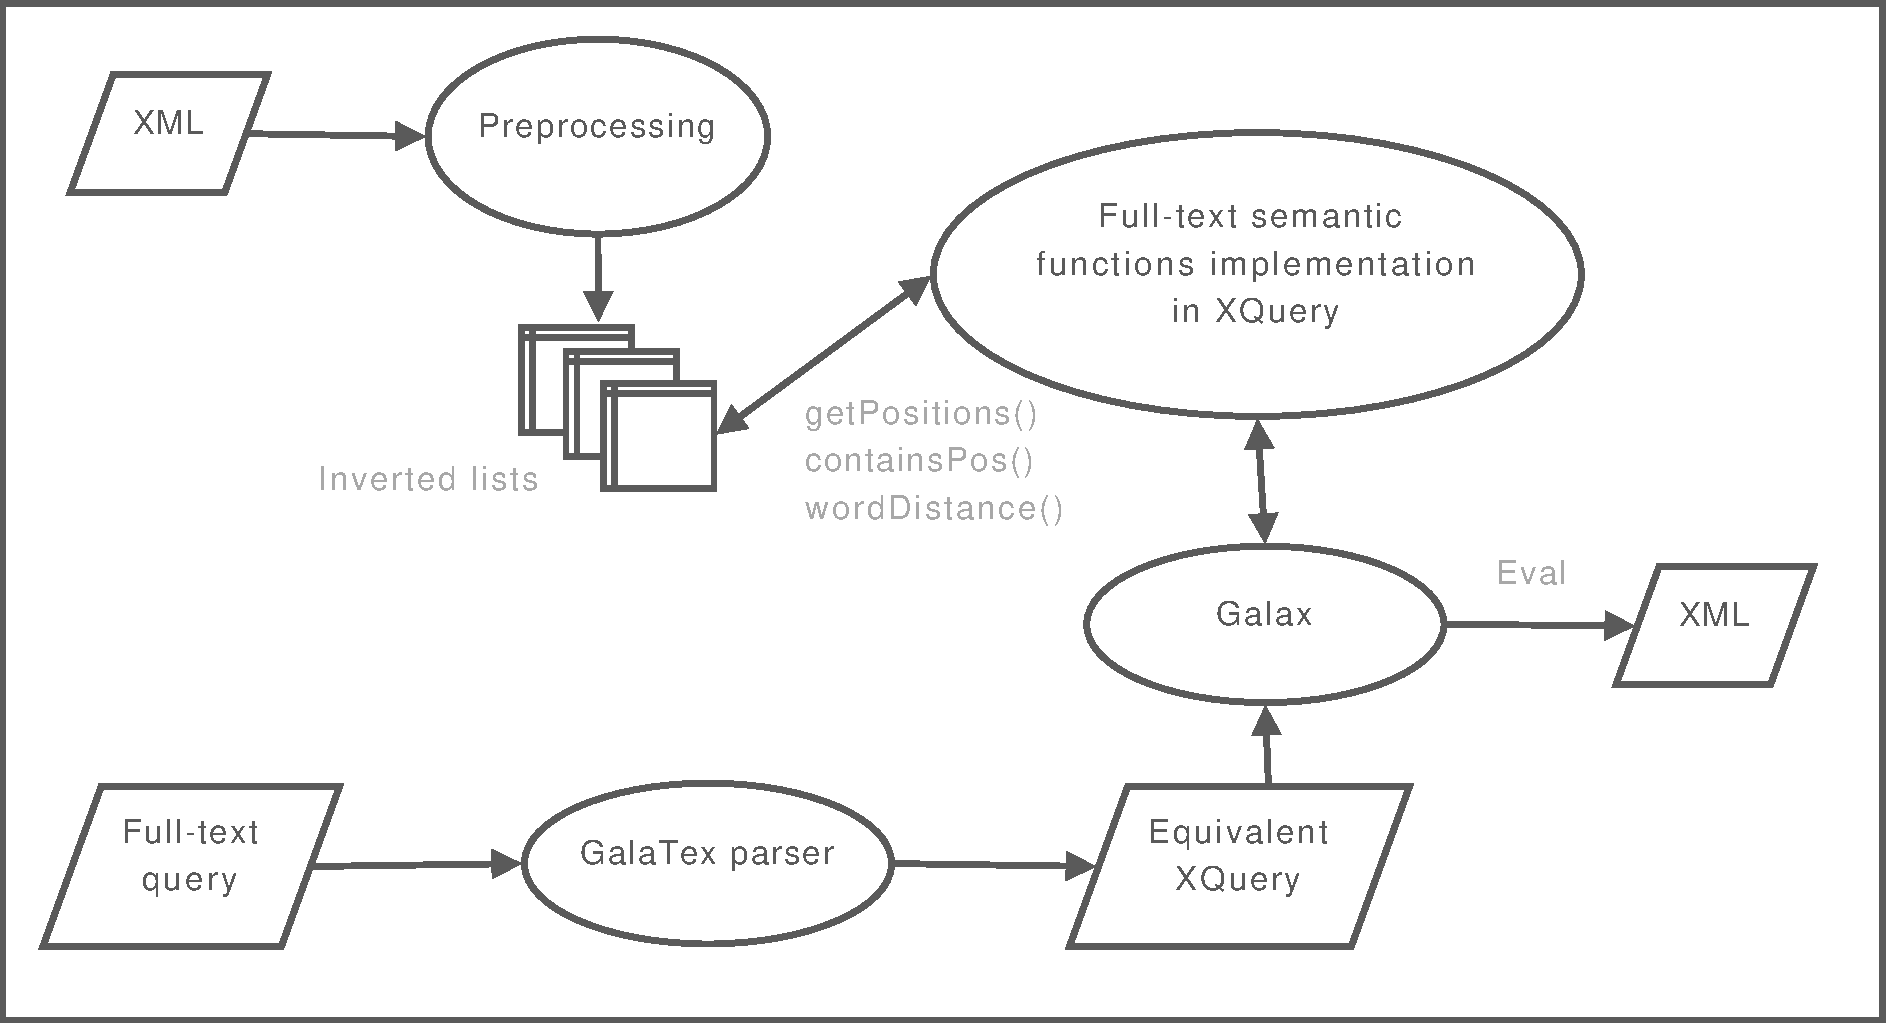
\includegraphics[width=1\textwidth]{diagrams/galatex_arch}
  \caption[GalaTex architecture]{Galatex architecture, based on architecture described on
  the GalaTex website\cite{galatex}}
  \label{figure:galatex:arch}
\end{figure}
Galatex is claimed to be the first full implementation of the W3C XQuery 1.0 
and XPath 2.0 Full-Text 1.0 specification\cite{w3c01}. As can be seen in figure
\ref{figure:galatex:arch}, Galatex translates the full-text parts of the query
into XQuery Core\cite{xquery_semantics} in the Galatex parser. The equivalent
XQuery query is then executed on the Galax query processor.

The most interesting aspect of Galatex is its full-text capabilities. This is
realised first and foremost by an implementation of the AllMatches data model
proposed by W3C\cite{w3c01}. Additionally, as mentioned above, the full-text fragments of the queries are
translanted into corresponding functions in regular XQuery. 

\subsection{Trait comparison matrix}
\label{sect:theory:existing_implementations:comparison}
This section will compare some important traits of the described
implementations, and will outline their implications.
\begin{table}[!h]
	\centering
	\begin{tabular}{ | p{3cm} | c | c | c |}
	\hline
	& eXist & Pathfinder & GalaTex \\ \hline
	Normalisation to XQuery Core & Yes & Yes & Yes \\ \hline
	Relational backend & No & Yes & No \\ \hline
	Full-text extensions & No & No & Yes \\ \hline
	Test suite coverage & 99.4\% & 99.4\% & n/a \\ \hline
	Free source code & Yes & Yes & Yes  \\
	\hline
	\end{tabular}
	\caption{Comparison of implementation traits}
	\label{figure:comparison_matrix}
\end{table}
The traits chosen for the comparison matrix in table
\ref{figure:comparison_matrix} are chosen due to their relevance to this
project. As can be seen, there is a spread in diversity across these
implementations. In particular, Pathfinder is the only implementation with a
relational backend. This implies that Pathfinder will be a natural focal point
of interest for studying existing methods of translation. As will be shown in
chapters \ref{chapter:method} and \ref{chapter:translation}, Pathfinder and
its loop lifting technique will serve as a basis for development of an
improved and novel translation method.